\documentclass[tikz,border=10pt]{standalone}
\usepackage{amsmath}
\begin{document}
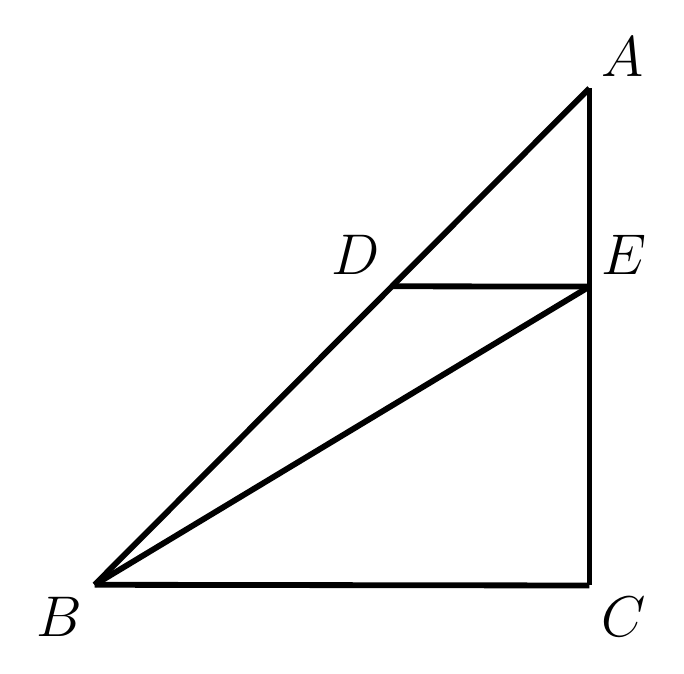
\begin{tikzpicture}[line join=round, line width=2.1pt]
\coordinate (A) at (3.144,3.171);
\coordinate (B) at (-3.140,-3.135);
\coordinate (C) at (3.144,-3.144);
\coordinate (D) at (0.640,0.656);



\coordinate (E) at (3.144,0.652);


\draw (A) -- (B);          
\draw (A) -- (E) -- (C);   
\draw (B) -- (C);          
\draw (B) -- (E);          
\draw (D) -- (E);          


\node[above right] at (A) {\fontsize{21}{25.2}\selectfont $A$};
\node[below left]  at (B) {\fontsize{21}{25.2}\selectfont $B$};
\node[below right] at (C) {\fontsize{21}{25.2}\selectfont $C$};
\node[above left]  at (D) {\fontsize{21}{25.2}\selectfont $D$};
\node[above right] at (E) {\fontsize{21}{25.2}\selectfont $E$};
\end{tikzpicture}
\end{document}